\documentclass[a4paper,12pt]{article}
\DeclareMathSizes{12}{30}{16}{12}

\usepackage[T1]{fontenc}
\usepackage[utf8]{inputenc}
\usepackage[english]{babel}

\usepackage[margin=3cm]{geometry}
\usepackage{graphicx}
\usepackage{blindtext}
\usepackage{titling}
\usepackage{titlesec}
\usepackage{caption}
\usepackage{wrapfig}
\usepackage{animate}

\titleformat{\section}
{\Large\bfseries}
{\Roman{section}.}
{0.5em}
{}

\titleformat{\subsection}
{\center\large\bfseries}
{\Roman{subsection}}
{0.5em}
{}

\titlespacing{\subsection}
{2em}{2.5em}{0.5em}

\title{Využití umělé inteligence a genetického algoritmu pro autonomní řízení}
\author{Marek Bečvář}
\date{Červen 2020}

\renewcommand{\maketitle}
{
    \begin{center}
        \vspace*{0cm}
        \LARGE{\textbf{\thetitle}}\\
        \vspace{0.5cm}
        \Large{\textbf{\theauthor}}\\
        \vspace{0.5cm}
        \normalsize{\thedate}
        \vspace{0.5cm}
        % \hline
    \end{center}
}

\addto\captionsenglish{\renewcommand{\figurename}{Schéma}}

\newcommand{\tab}
{
    \hspace*{1em}
}

\begin{document}
    \maketitle

    \vspace{0.5cm}

    % \animategraphics[controls=play,loop]{20}{gif1/clever_anim-}{0}{100}

    \section{O projektu}
        \tab Tento projekt byl zpracován v roce 2020 jako maturitní práce 6.ročníku 
        víceletého gymnázia Boženy Němcové v Hradci Králové.\\
        \tab Hlavní myšlenkou je využití strojového učení umělé inteligence genetickým 
        algoritmem s cílem projetí uživatelem nastavené tratě. Výsledek snažení 
        je postupně promítán do grafu. Schopnost by se měla, i po dosažení cíle (projetí tratí),
        stále rozvíjet.

    \section{Funkce}
    \subsection{Umělá inteligence}
        Pojem \textbf{umělé inteligence} je dnes člověku prezentován v trochu zkreslené formě.
        Lidem se mohou vybavit některé sci-fi filmové scény s roboty, ale to není úplně přesné.
        Ve slově \textit{inteligence} se doopravdy skrývá řada výpočtů zpracovávajících vstupní data 
        na požadovaný výstup. Tyto výpočty se provádějí v předem definované 
        struktuře tzv. \textbf{neuronové sítě}.\\
            
        \begin{figure}[h]
        \centering
        \begin{minipage}{.5\textwidth}
            \centering
            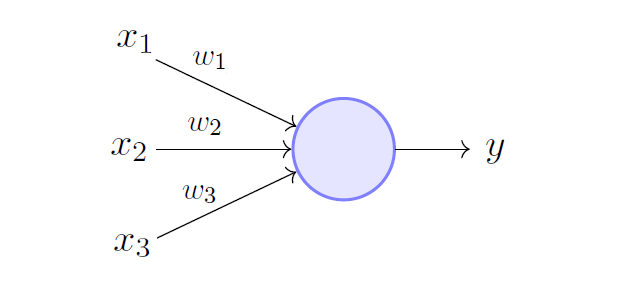
\includegraphics[width=1.1\linewidth]{data/perceptron-model1.png}
            \captionof{figure}{Perceptron}
            \label{fig:perceptron}
        \end{minipage}%
        \begin{minipage}{.5\textwidth}
            \centering
            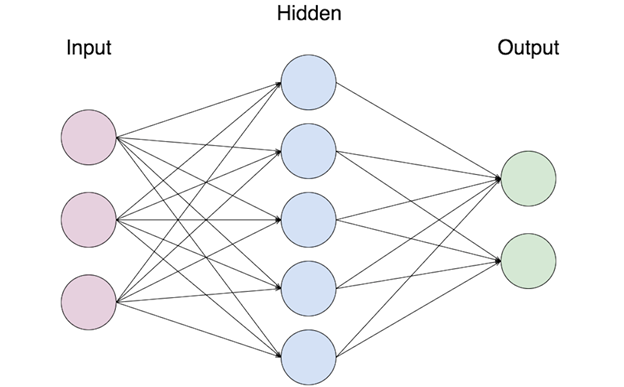
\includegraphics[width=1.1\linewidth]{data/easynn-scheme.png}
            \captionof{figure}{Neuronová síť}
            \label{fig:easynn}
        \end{minipage}
        \end{figure}

        Neuronová síť je modelována s inspirací v mozkových neuronech. Každý bod je považován za
        samostatný neuron a má řadu spojení, z biologie \textit{axonů}. Právě tato spojení jsou hlavní
        funkční složkou neuronových sítí, v programu tedy vždy uchováváme číselnou hodnotu každého z nich. 
        Tato hodnota je obvykle reálné číslo v rozsahu od -1 do 1.
        Neurony dělíme do vrstev (VSTUP, SKRYTÁ, VÝSTUP). Existuje pravidlo, že každý neuron z nižší vrstvy 
        je spojen se všemi neurony ve vyšší vrstvě. Nejjednodušším znázorněním je 
        právě Schéma~\ref{fig:perceptron}, skládající se z 3 vstupů a 1 výstupu.
        Jak se ale tvoří číselné hodnoty?

        \begin{equation}
            \sigma(\displaystyle\sum_{k=1}^{n}{x_k * w_k})
        \end{equation}
        kde $\sigma$ je \textit{aktivační funkce}. Tyto funkce pouze upravují možný rozsah výstupních 
        hodnot.
        \begin{wrapfigure}{r}{0.45\textwidth}
            \centering
            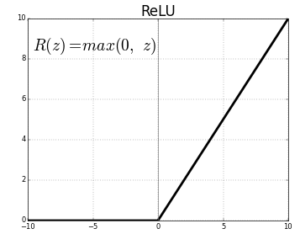
\includegraphics[width=0.8\linewidth]{data/relu.png}
            \caption{RELU aktivační funkce} 
            \label{fig:relu}
        \end{wrapfigure}

        \vspace{0.75cm}Příkladem takové aktivační funkce může být třeba RELU (Rectified Linear Unit).
        Ta výstupní hodnoty změní tak, že kladné nechá beze změny a záporné změní na nulu.
        Tyto změny pomáhají při přenosu signálu mezi neurony v síti.
        \\\\\\\\\\\\
        Složitější neuronové sítě jsou už jen opakováním tohoto zavedeného postupu. Dále se pro sítě 
        zavádí jméno hluboké neuronové sítě (\textit{z ang. deep neural network}). 
        To označuje schéma, ve kterém je použita více než jedna skrytá vrstva.
        \begin{figure}[h]
            \centering
            \centering
            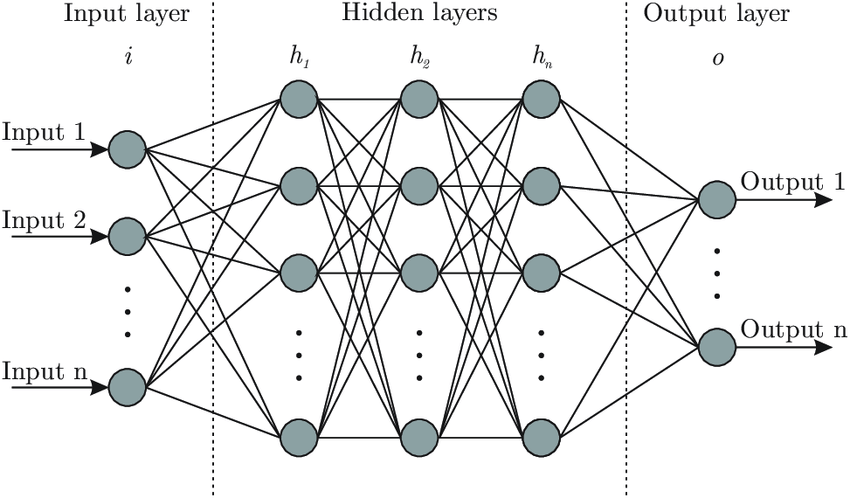
\includegraphics[width=0.76\textwidth]{data/nn-scheme.png}
            \captionof{figure}{Hluboká neuronová síť}
            \label{fig:deepnn}
        \end{figure}

    \subsection{Genetický algoritmus}
\end{document}
